% LINEAR SYSTEMS AND CONTROL
% Homework 2 : 

\documentclass[10pt,a4paper]{article}
\usepackage[latin1]{inputenc}
\usepackage{amsmath}
\usepackage{amsfonts}
\usepackage{amssymb}
\usepackage{graphics} 
\usepackage{graphicx}
\usepackage{float}
\usepackage{subfigure}

\usepackage{trfsigns}
\author{Ana Huaman}
\title{\textbf{Homework 2} \\ ECE 6550: Linear Control and Systems}
\begin{document}
\maketitle

%%%%%%%%%%%%%%%%%%%%%%%%%%%%%%%%%%%%%%%%%
% Question 1
%%%%%%%%%%%%%%%%%%%%%%%%%%%%%%%%%%%%%%%%%
\section{}
Given a matrix $A$, whose characteristic polynomial is given by

\[ \lambda^{n} + a_{n-1}\lambda^{n-1}+...+a_{1}\lambda + a_{0} \]

\subsection*{a}
Assuming that $A^{-1}$ exists, use the Cayley-Hamilton theorem to derive an expression for the inverse, using the polynomial above.

\subsection*{Solution}

From Cayley-Hamilton, if we have the characteristic polynomial defined with:

\[ \lambda^{n} + a_{n-1}\lambda^{n-1}+...+a_{1}\lambda + a_{0} \]

Then, the following is valid:

\begin{equation} 
A^{n} + a_{n-1}A^{n-1}+...+a_{1}A + a_{0}I  = 0
\label{Eq:P1a-Cayley}
\end{equation}

Let's rearrange the expression in (\ref{Eq:P1a-Cayley}) by leaving $a_{0}$ in the left side:

\[ a_{0}I = - \left ( a_{1}A + ... + a_{n-1}A^{n-1} + A^{n} \right ) \]

Now, assuming that $A^{-1}$ exists, multiply both sides with it:

\[ a_{0}IA^{-1} = - \left ( a_{1}AA^{-1} + ... + a_{n-1}A^{n-1}A^{-1} + A^{n}A^{-1} \right ) \]

Multiplying:

\[ a_{0}A^{-1} = - \left ( a_{1}I + ... + a_{n-1}A^{n-2} + A^{n-1} \right ) \]

Then we have an expression for $A^{-1}$:
\smallskip
\begin{center}
\fbox{$A^{-1} = - \dfrac{1}{a_{0}}\left ( a_{1}I + ... + a_{n-1}A^{n-2} + A^{n-1} \right )$}
\end{center}

% ----------------------------------------
\subsection*{b}
Let $A$ be the $2 \times 2$ matrix

\[ A = 
   \begin{bmatrix}
   a & b \\
   c & d
   \end{bmatrix} 
\]

Using your result in $1a$, derive an explicit expression for $A^{-1}$

\subsection*{Solution}
First, let's find the characteristic polynomial:

\[P(\lambda) = 
\left | 
\lambda I - A
\right | 
\]
\[P(\lambda) = 
\left | 
\begin{matrix}
\lambda -a & -b \\
-c & \lambda - d
\end{matrix}
\right | 
\]

\[P(\lambda) = \lambda^{2} - (a+d)\lambda + (ad-bc) \]

Now, we have the coefficients:

$a_{0} = (ad-bc)$, \hspace*{1cm} $a_{1} = -(a+d)$

Okay, now back to our matrix inverse. Using the result in \textbf{a} for $n = 2$, we can calculate the inverse as:

\[ A^{-1} = - \dfrac{1}{a_{0}}\left ( a_{1}I +  A^{2-1} \right ) \]
\[ A^{-1} = - \dfrac{1}{a_{0}}\left ( a_{1}I + A \right ) \]

Replacing the coefficients, we have:

\[ A^{-1} = - \dfrac{1}{ad-bc}\left ( -(a+d)I + A \right ) \]
\[ A^{-1} = - \dfrac{1}{ad-bc}\left ( 
\begin{bmatrix}
-(a+d) & 0 \\
0 & -(a+d)
\end{bmatrix}
 +  
 \begin{bmatrix}
a & b \\
c & d
\end{bmatrix}
\right ) \]

\[ A^{-1} = - \dfrac{1}{ad-bc}\left ( 
\begin{bmatrix}
-(a+d) + a & 0+b \\
 0+c & -(a+d)+d
\end{bmatrix}
\right ) \]

\[ A^{-1} = - \dfrac{1}{ad-bc}\left ( 
\begin{bmatrix}
-d & b \\
 c & -a
\end{bmatrix}
\right ) \]

\[ A^{-1} = \dfrac{1}{ad-bc}\left ( 
\begin{bmatrix}
d & -b \\
-c & a
\end{bmatrix}
\right ) \]

%%%%%%%%%%%%%%%%%%%%%%%%%%%%%%%%%%%%%%%%%
% Question 2
%%%%%%%%%%%%%%%%%%%%%%%%%%%%%%%%%%%%%%%%%
\section{}
Read Chapter/Lecture 7 in the textbook (available on T-Square under resources/JordanChapter.pdf). Using your newfound knowledge, find
\[ e^{At} \]

for the matrix

\[ A = 
\begin{bmatrix}
5 & 4 & 2 & 1 \\
0 & 1 & -1 & -1 \\
-1 & -1 & 3 & 0 \\
1 & 1 & -1 & 2
\end{bmatrix}
\]

(Note: It is enough if you write down the matrices you need to multiply - you do not actually have to explicitly carry out the rather tedious multiplications)

\subsection*{Solution}
From the hint that our generous instructor put in our homework sheet, we know that:

\[ J = PAP^{-1} \]

Now beware! Because Matlab actually gives you $P^{-1}$. Hence, replacing properly here and there:

\[ J = PAP^{-1} \]
\[
J = 
\begin{bmatrix}
   0 &  1 &  1 &  1 \\
   0 &  0 &  1 &  1 \\ 
   0 &  0 & -1 &  0 \\
   1 &  1 &  1 &  0
\end{bmatrix}
\begin{bmatrix}
   5 &  4 &  2 &  1 \\
   0 &  1 & -1 & -1 \\
  -1 & -1 &  3 &  0 \\
   1 &  1 & -1 &  2
\end{bmatrix}
\begin{bmatrix}
  -1 &  1 &  1 & 1 \\
   1 & -1 &  0 & 0 \\
   0 &  0 & -1 & 0 \\
   0 &  1 &  1 & 0 
\end{bmatrix}
\]

\[ J = 
\begin{bmatrix}
   1 &  0 &  0 &  0 \\
   0 &  2 &  0 &  0 \\
   0 &  0 &  4 &  1 \\
   0 &  0 &  0 &  4
\end{bmatrix}
\]

where $J$ is formed by $3$ jordan blocks:

\begin{center}
$J_{1} = 1$, $J_{2} = 2$ and $J_{3} = \begin{bmatrix}4 & 1 \\ 0 & 4\end{bmatrix}$ 
\end{center}

Now, to find $e^{At}$, from the book's definition, we know that we have to calculate:

\begin{equation}
e^{At} = P^{-1}
\begin{bmatrix}
e^{J_{1}t} & 0 & 0 \\
0 & e^{J_{2}t} & 0 \\
0 & 0 & e^{J_{3}t}  
\end{bmatrix}
P
\label{Eq:P2-expAt}
\end{equation}

From the book again, we calculate the exponential for each of our jordan blocks:

\[ e^{J_{1}t} = e^{1t} \]
\[ e^{J_{2}t} = e^{2t} \]
\[ e^{J_{3}t} = 
e^{4t}
\begin{bmatrix}1 & t \\ 0 & 1\end{bmatrix}
=
\begin{bmatrix}e^{4t} & te^{4t} \\ 0 & e^{4t}\end{bmatrix}
\] 

Putting it all together, we replace it in (\ref{Eq:P2-expAt}):
\[
e^{At} = P^{-1}
\begin{bmatrix}
e^{1t} & 0 & 0 & 0 \\
0 & e^{2t} & 0 & 0 \\
0 & 0 & e^{4t} & te^{4t} \\
0 & 0 & 0 & e^{4t}  
\end{bmatrix}
P
\]

So we finally have this expression:
\begin{center}
\fbox{$e^{At} = \begin{bmatrix}
  -1 &  1 &  1 & 1 \\
   1 & -1 &  0 & 0 \\
   0 &  0 & -1 & 0 \\
   0 &  1 &  1 & 0 
\end{bmatrix}
\begin{bmatrix}
e^{1t} & 0 & 0 & 0 \\
0 & e^{2t} & 0 & 0 \\
0 & 0 & e^{4t} & te^{4t} \\
0 & 0 & 0 & e^{4t}  
\end{bmatrix}
\begin{bmatrix}
   0 &  1 &  1 &  1 \\
   0 &  0 &  1 &  1 \\ 
   0 &  0 & -1 &  0 \\
   1 &  1 &  1 &  0
\end{bmatrix}$}
\end{center}

%%%%%%%%%%%%%%%%%%%%%%%%%%%%%%%%%%%%%%%%%
% Question 3
%%%%%%%%%%%%%%%%%%%%%%%%%%%%%%%%%%%%%%%%%
\section{}
Let
\begin{center}
$ \dot{x}(t) = 
\begin{bmatrix}
\cos(t) & t \\
t & \cos(t)
\end{bmatrix}
x(t)$, \hspace*{1cm}
$x(t_{0}) = x_{0}$
\end{center}

What is $x(t)$?

\subsection*{Solution}

Let\'s see if we can apply an special rule we saw in class. This rule says that:

If $A(t)A(\tau) = A(\tau)A(t)$ then:

\[ \Phi (t,t_{0}) = e^{ \int_{t_{0}}^{t}A(\tau)d\tau } \]

Checking if our $A(t)$ verifies this:

\[A(t)A(\tau) = 
\begin{bmatrix}
\cos (t) & t \\
t & \cos (t)
\end{bmatrix}
\begin{bmatrix}
\cos (\tau) & \tau \\
\tau & \cos (\tau)
\end{bmatrix}
=
\begin{bmatrix}
\cos (t)\cos (\tau) + t\tau & \cos (t)\tau + t\cos (\tau) \\
t\cos (\tau) + \cos (t)\tau & t\tau + \cos (t)\cos (\tau)
\end{bmatrix}
\]

\[A(\tau)A(t) = 
\begin{bmatrix}
\cos (\tau) & \tau \\
\tau & \cos (\tau)
\end{bmatrix}
\begin{bmatrix}
\cos (t) & t \\
t & \cos (t)
\end{bmatrix}
=
\begin{bmatrix}
\cos (\tau)\cos (t) + \tau t & \cos (\tau)t + \tau\cos (t) \\
\tau\cos (t) + \cos (\tau)t & \tau t + \cos (\tau)\cos (t)
\end{bmatrix}
\]

Yay! We can see that $A(t)A(\tau) = A(\tau)A(t)$, then we proceed to calculate $\Phi(t,t_{0})$

\[ \Phi (t,t_{0}) = e^{ \displaystyle \int_{t_{0}}^{t}A(\tau)d\tau } \]
\[ \Phi (t,t_{0}) = e^{ \displaystyle \int_{t_{0}}^{t}
\begin{bmatrix}
\cos (\tau) & \tau \\
\tau & \cos (\tau)
\end{bmatrix}
d\tau } \]

\[ \Phi (t,t_{0}) = e^{ 
\begin{bmatrix}
\sin (\tau) & \tau^{2}/2 \\
\tau^{2}/2 & \sin (\tau)
\end{bmatrix} \Bigg | _{t_{0}}^{t} } 
\]

\begin{equation} 
\Phi (t,t_{0}) = e^{ 
\begin{bmatrix}
\sin (t) & t^{2}/2 \\
t^{2}/2 & \sin (t)
\end{bmatrix} } 
\times
e^{ -
\begin{bmatrix}
\sin (t_{0}) & t_{0}^{2}/2 \\
t_{0}^{2}/2 & \sin (t_{0})
\end{bmatrix} }
\label{Eq:P3-PhiEq}
\end{equation}

Both exponentials have the same form so I will solve for the one depending on $t$ first. Then our problem is reduced to find:
\[ e^{ 
\begin{bmatrix}
\sin (t) & t^{2}/2 \\
t^{2}/2 & \sin (t)
\end{bmatrix} }
= e^{B} 
\]

Calling $B$ to the matrix in the exponent. Since this form is not easy to solve, we first find the eigenvalues and eigenvectors of $B$, in order to get an easier computation. Calculating we obtain that the eigenvalues are:

\[ \lambda_{1}(B) = \sin (t) + t^{2}/2  \rightarrow \upsilon_{1}(B) = \begin{bmatrix}1 & 1 \end{bmatrix}^{T} \]
\[ \lambda_{2}(B) = \sin (t) - t^{2}/2  \rightarrow \upsilon_{2}(B) = \begin{bmatrix}1 & -1 \end{bmatrix}^{T} \]

So, we can construct the matrix $V$ with the eigenvectors as columns:

\[ V =
\begin{bmatrix}
1 & 1 \\ 
1 & -1
\end{bmatrix}
\]

Such that:
 
\[ V^{-1}BV =
\dfrac{1}{2} 
\begin{bmatrix}
1 & 1 \\ 
1 & -1
\end{bmatrix}
\begin{bmatrix}
\sin (t) & t^{2}/2 \\
t^{2}/2 & \sin (t)
\end{bmatrix} 
\begin{bmatrix}
1 & 1 \\ 
1 & -1
\end{bmatrix}
\]
\[ V^{-1}BV =
\begin{bmatrix}
\sin (t) + t^{2}/2 & 0 \\
0 & \sin (t) - t^{2}/2
\end{bmatrix}
\]

Now, since we know that:

\[ V^{-1}e^{B}V = e^{V^{-1}BV} \]
\[ e^{B} = Ve^{V^{-1}BV}V^{-1} \]

Replacing what we know:
\[ e^{B} = 
\dfrac{1}{2} 
\begin{bmatrix}
1 & 1 \\ 
1 & -1
\end{bmatrix}
e^{\begin{bmatrix}
\sin (t) + t^{2}/2 & 0 \\
0 & \sin (t) - t^{2}/2
\end{bmatrix}}
\begin{bmatrix}
1 & 1 \\ 
1 & -1
\end{bmatrix}
\]

Since the exponential in the middle has a diagonal matrix, it is easy to compute:
\[ e^{B} = 
\dfrac{1}{2} 
\begin{bmatrix}
1 & 1 \\ 
1 & -1
\end{bmatrix}
\begin{bmatrix}
e^{\sin (t) + t^{2}/2} & 0 \\
0 & e^{\sin (t) - t^{2}/2}
\end{bmatrix}
\begin{bmatrix}
1 & 1 \\ 
1 & -1
\end{bmatrix}
\]

Multiplying the whole thing, we get:
\[ e^{B} =
\dfrac{1}{2} 
\begin{bmatrix}
e^{\sin (t) + t^{2}/2} + e^{\sin (t) - t^{2}/2} & e^{\sin (t) + t^{2}/2} - e^{\sin (t) - t^{2}/2} \\
e^{\sin (t) + t^{2}/2} - e^{\sin (t) - t^{2}/2} & e^{\sin (t) + t^{2}/2} + e^{\sin (t) - t^{2}/2}
\end{bmatrix}
\]

Yay again! We can replace this on (\ref{Eq:P3-PhiEq}), getting:
\[
\Phi (t,t_{0}) = 
\dfrac{1}{2} 
\begin{bmatrix}
e^{\sin (t) + t^{2}/2} + e^{\sin (t) - t^{2}/2} & e^{\sin (t) + t^{2}/2} - e^{\sin (t) - t^{2}/2} \\
e^{\sin (t) + t^{2}/2} - e^{\sin (t) - t^{2}/2} & e^{\sin (t) + t^{2}/2} + e^{\sin (t) - t^{2}/2}
\end{bmatrix}
\times
e^{ -
\begin{bmatrix}
\sin (t_{0}) & t_{0}^{2}/2 \\
t_{0}^{2}/2 & \sin (t_{0})
\end{bmatrix} }
\]

The second factor (depending on $t_{0}$) has a similar form to the one we just calculated. Hence, I will not repeat the math and write the expression:
\medskip

\fbox{
$\Phi (t,t_{0}) = 
\dfrac{1}{2} 
\begin{bmatrix}
e^{\sin (t) + t^{2}/2} + e^{\sin (t) - t^{2}/2} & e^{\sin (t) + t^{2}/2} - e^{\sin (t) - t^{2}/2} \\
e^{\sin (t) + t^{2}/2} - e^{\sin (t) - t^{2}/2} & e^{\sin (t) + t^{2}/2} + e^{\sin (t) - t^{2}/2}
\end{bmatrix}
\times
E(t_{0})$ }

where:
\[ E(t_{0}) =
\dfrac{1}{2} 
\begin{bmatrix}
e^{-\sin (t_{0}) - t_{0}^{2}/2} + e^{-\sin (t_{0}) + t_{0}^{2}/2} & e^{-\sin (t) - t^{2}/2} - e^{-\sin (t) + t^{2}/2} \\
e^{-\sin (t) - t^{2}/2} - e^{-\sin (t) + t^{2}/2} & e^{-\sin (t) - t^{2}/2} + e^{-\sin (t) + t^{2}/2}
\end{bmatrix}
\]

So, finally (phew!) we can replace this in the general solution:

\[x(t) = \Phi (t,t_{0}) x_{0} \]

\fbox{
$ x(t) = 
\dfrac{1}{2} 
\begin{bmatrix}
e^{\sin (t) + t^{2}/2} + e^{\sin (t) - t^{2}/2} & e^{\sin (t) + t^{2}/2} - e^{\sin (t) - t^{2}/2} \\
e^{\sin (t) + t^{2}/2} - e^{\sin (t) - t^{2}/2} & e^{\sin (t) + t^{2}/2} + e^{\sin (t) - t^{2}/2}
\end{bmatrix}
\times
E(t_{0})
\times
x_{0}$ }

\medskip

Just replace the $E(t_{0})$ we found a few lines above and presto!

%%%%%%%%%%%%%%%%%%%%%%%%%%%%%%%%%%%%%%%%%
% Question 4
%%%%%%%%%%%%%%%%%%%%%%%%%%%%%%%%%%%%%%%%%
\section{}
Let

\[ \dot{x} =
\begin{bmatrix}
-1 & 1 \\
0 & -1
\end{bmatrix}x + 
\begin{bmatrix}
1 \\
0
\end{bmatrix}u
\]

We want to implement this as a discrete time, sampled-data system. In other words, find the matrices $\hat{A}$ and $\hat{B}$ such that the discrete-time system is given exactly by

\[ x_{k+1} = \hat{A}x_{k} + \hat{B}u_{k} \]

(You may assume that the sample time is $\delta$)
% ---------------------------
\subsection*{Solution}
From theory, we have the following expressions for $\hat{A}$ and $\hat{B}$:
\begin{equation} 
\begin{matrix}
\hat{A} = e^{A \delta} \\
\hat{B} = \displaystyle \int_{0}^{\delta} e^{A(\delta - \tau)}Bd\tau 
\end{matrix}
\label{Eq:P4-General}
\end{equation}

And from our problem we have:
\begin{center}
$A = \begin{bmatrix}-1 & 1 \\ 0 & -1 \end{bmatrix}$ and $B = \begin{bmatrix} 1 \\ 0 \end{bmatrix}$
\end{center}

Now, check out $A$. It happens to have the form of a Jordan block, right? Just to be sure, let us calculate its eigenvalues:
\begin{center}
$ \lambda_{1}(A) = -1$ with multiplicity 2
\end{center}

Now, we know that for a Jordan block $J$, the calculation of $e^{Jt}$ is straightforward:

\[ e^{Jt} = e^{\lambda t}\begin{bmatrix}1 & t \\ 0 & 1 \end{bmatrix} \]

Replacing properly for our case (where $J$ happens to be $A$ and using $\delta$ instead of $t$:

\[ e^{A\delta} = e^{-1\delta}\begin{bmatrix}1 & \delta \\ 0 & 1 \end{bmatrix} \]

\begin{equation} 
e^{A\delta} = \begin{bmatrix}e^{-\delta} & \delta e^{-\delta} \\ 0 & e^{-\delta} \end{bmatrix} 
\label{Eq:P4-eAd}
\end{equation}

So we can replace (\ref{Eq:P4-eAd})  and $B = \begin{bmatrix} 1 & 0 \end{bmatrix}^{T}$ in (\ref{Eq:P4-General}), obtaining:

\[
\begin{matrix}
\hat{A} = \begin{bmatrix}e^{-\delta} & \delta e^{-\delta} \\ 0 & e^{-\delta} \end{bmatrix}  \\
\hat{B} = \displaystyle \int_{0}^{\delta} \begin{bmatrix}e^{-(\delta - \tau)} & te^{-(\delta - \tau)} \\ 0 & e^{-(\delta - \tau)} \end{bmatrix}\begin{bmatrix} 1 \\ 0 \end{bmatrix}d\tau 
\end{matrix}
\]

Further, $B$ is:

\[ \hat{B} = \displaystyle \int_{0}^{\delta} \begin{bmatrix}e^{-(\delta - \tau)} \\ 0\end{bmatrix}d\tau \]
\[ \hat{B} = \begin{bmatrix}e^{\tau - \delta} \\ 0\end{bmatrix} \Bigg |_{0}^{\delta} \rightarrow \hat{B} = \begin{bmatrix} 1 - e^{-\delta} \\ 0\end{bmatrix}  \]

Our problem is solved!:

\begin{center}
\fbox{$\hat{A} = \begin{bmatrix}e^{-\delta} & \delta e^{-\delta} \\ 0 & e^{-\delta} \end{bmatrix}$}
\fbox{$\hat{B} = \begin{bmatrix} 1 - e^{-\delta} \\ 0\end{bmatrix}$}
\end{center}



%%%%%%%%%%%%%%%%%%%%%%%%%%%%%%%%%%%%%%%%%
% Question 5
%%%%%%%%%%%%%%%%%%%%%%%%%%%%%%%%%%%%%%%%%
\section{}
Use the $A$,$B$,$\hat{A}$, $\hat{B}$ matrices from Question 4. Let

\begin{center}
$y_{k} = 
\begin{bmatrix}
0 & 1
\end{bmatrix}
x$, \hspace*{1cm}
$x(0)
=
\begin{bmatrix}
0.1 \\
0.1
\end{bmatrix}
$, \hspace*{1cm}
$u_{k} = e^{-k\delta}$
\end{center}

Go to T-Square under Resources/m-files and download the MatLab file\textbf{ExactVsApprox.m} and insert your $\hat{A}$ and $\hat{B}$ matrices. Plot your solutions for different $\delta$ values. When do the approximate and exact solutions start to differ?
% -------------------------
\subsection*{Solution}
We plotted the results for 6 values of $\delta$ such as: $\{0.05, 0.1, 0.2, 0.4, 0.8, 1.0\}$. As it is expected, the smaller the $\delta$ the better the approximation, since the Higher terms of the Taylor expansion go quicker to zero (making the approximation more accurate).

From the plots below, I can observe that:
(Note: The graph "on top" is the exact one, the one  "below" is the approximate. In the pdf they appear in color)
\begin{itemize}
\item{$\delta = 0.05$:  Both graphs are nearly the same. The small error is noticeable in the curved part of the plots }
\item{$\delta = 0.1$: The error extends along the curved section of the plots, but still both plots do not show a significant difference (in my opinion :)}
\item{$\delta = 0.2$: The error is now quite evident and runs nearly until $y=0$ (around $k = 25$)}
\item{$\delta = 0.4, 0.6, 0.8$: The error is simply big. For $\delta = 0.8$ in fact we can see that the approximation is not good at all (the approximated plot look nearly as a vertical line in the curved section.}
\end{itemize}
 
So, from the plots I think that I would use a $\delta = 0.05$ at most. Of course it would be better to use smaller values, but it seems to me that $\delta = 0.05$ should still work fine.
\smallskip
 
And now here the plots!

 
\begin{center}
	\begin{figure}[H]
			  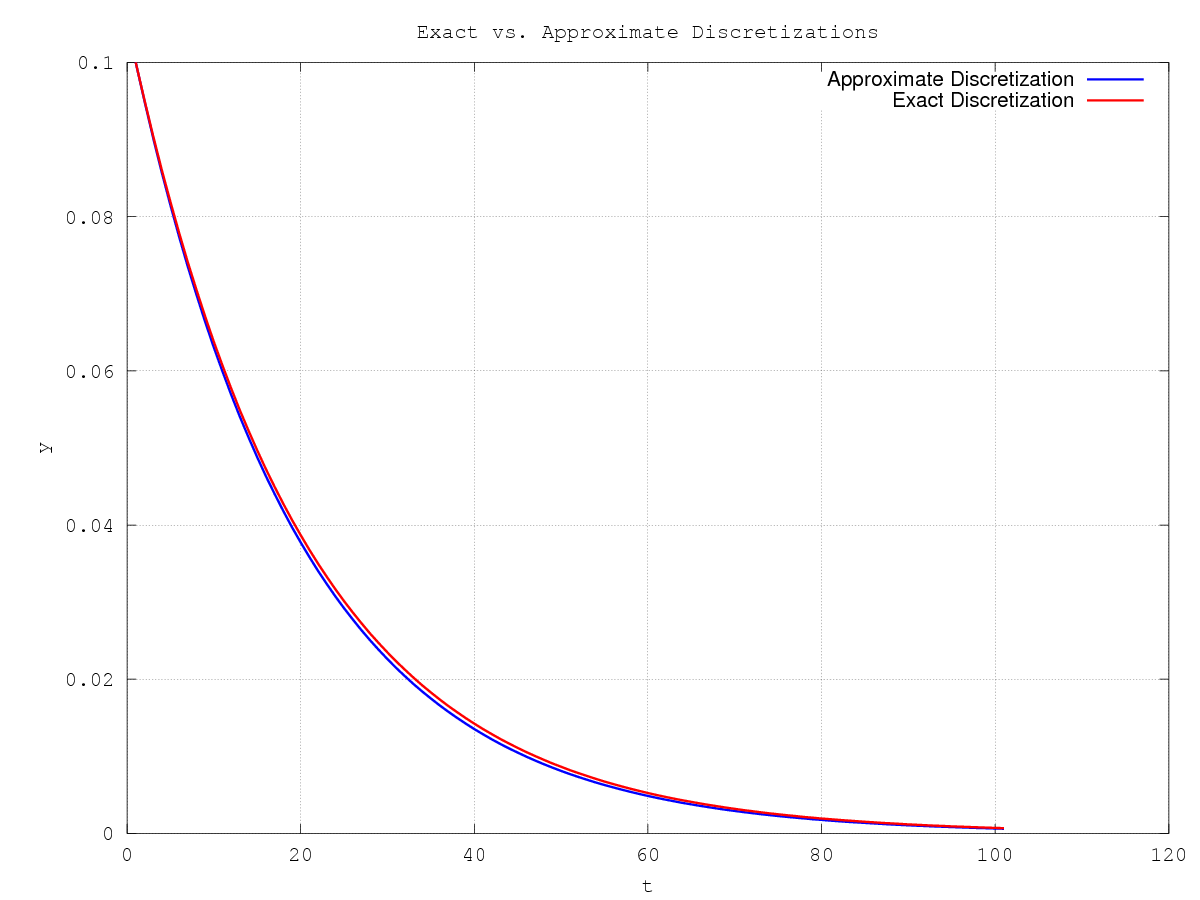
\includegraphics[scale=0.5]{figures/Question5Delta005.png} 
	          \label{fig:Q5Delta1}
	\caption{ $\delta = 0.05$  seconds}
	\end{figure}
	
	\begin{figure}[H]
			  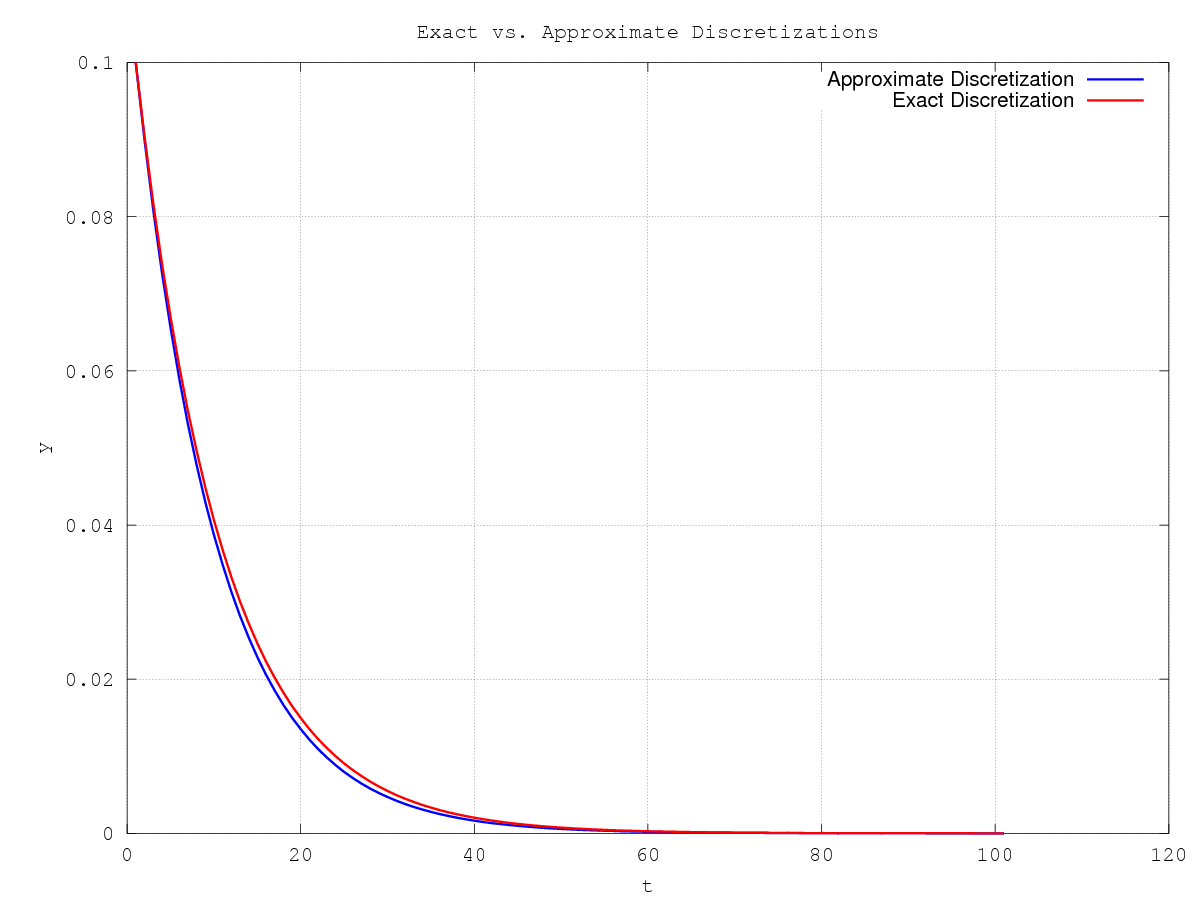
\includegraphics[scale=0.5]{figures/Question5Delta01.png} 
	          \label{fig:Q5Delta2}
	\caption{ $\delta = 0.1$  seconds}
	\end{figure}

	\begin{figure}[H]
			  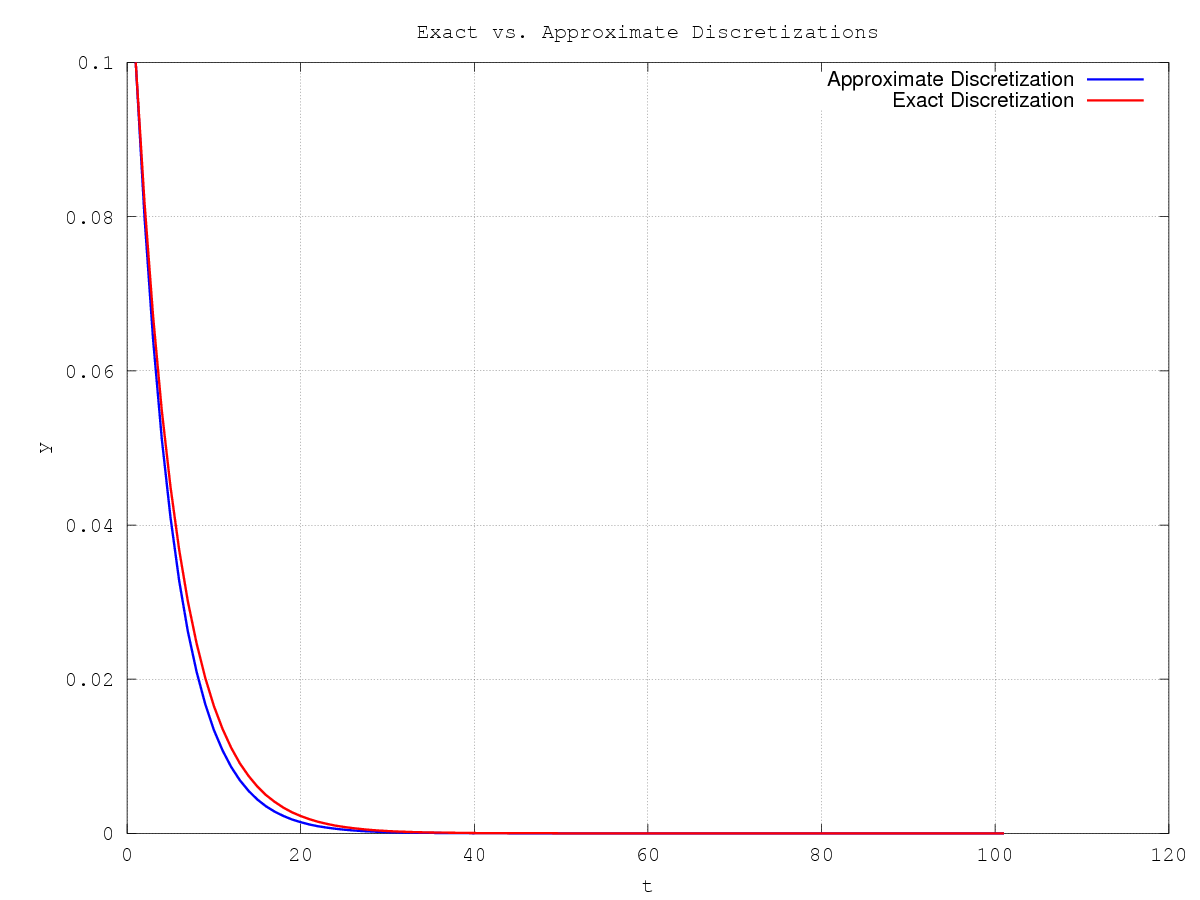
\includegraphics[scale=0.5]{figures/Question5Delta02.png} 
	          \label{fig:Q5Delta3}
	\caption{ $\delta = 0.2$  seconds}
	\end{figure}

	\begin{figure}[H]
			  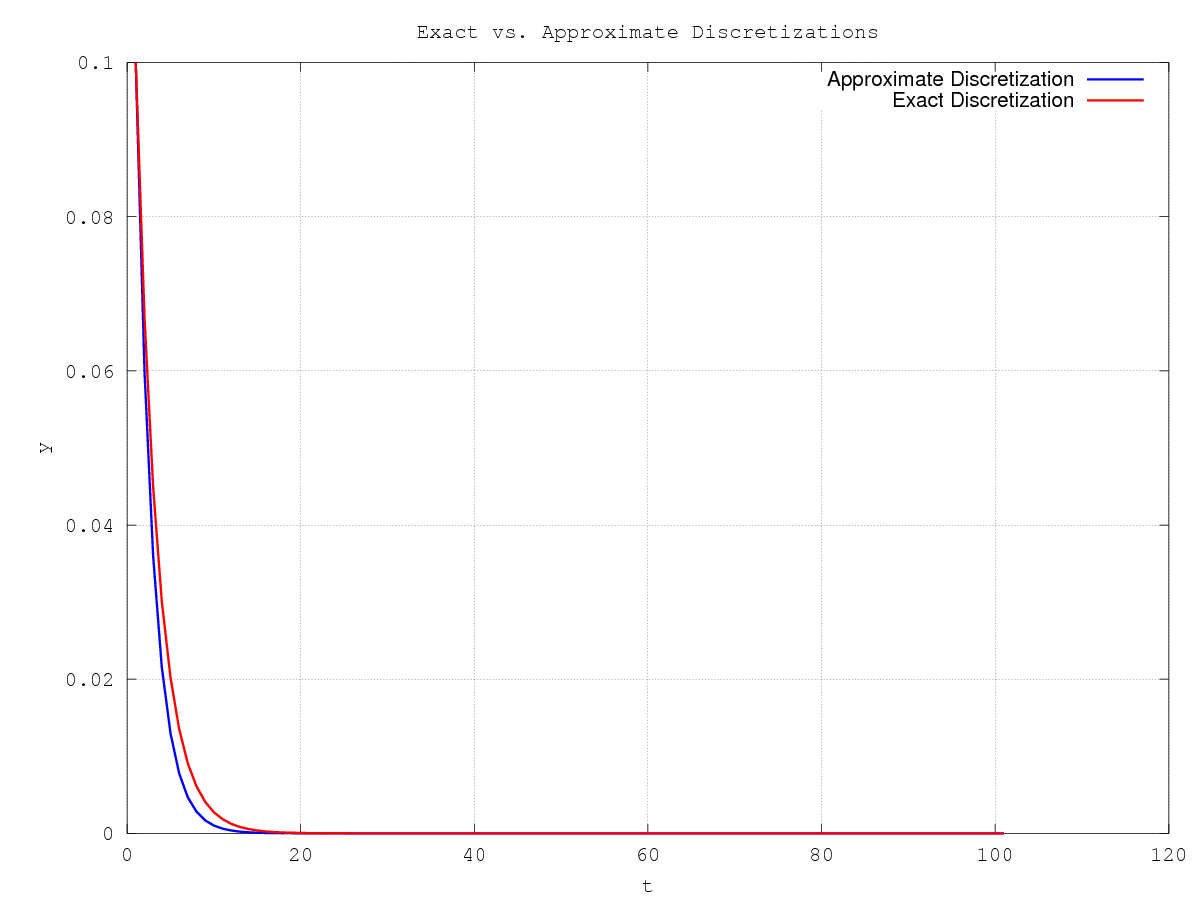
\includegraphics[scale=0.5]{figures/Question5Delta04.png} 
	          \label{fig:Q5Delta4}
	\caption{ $\delta = 0.4$  seconds}
	\end{figure}

	\begin{figure}[H]
			  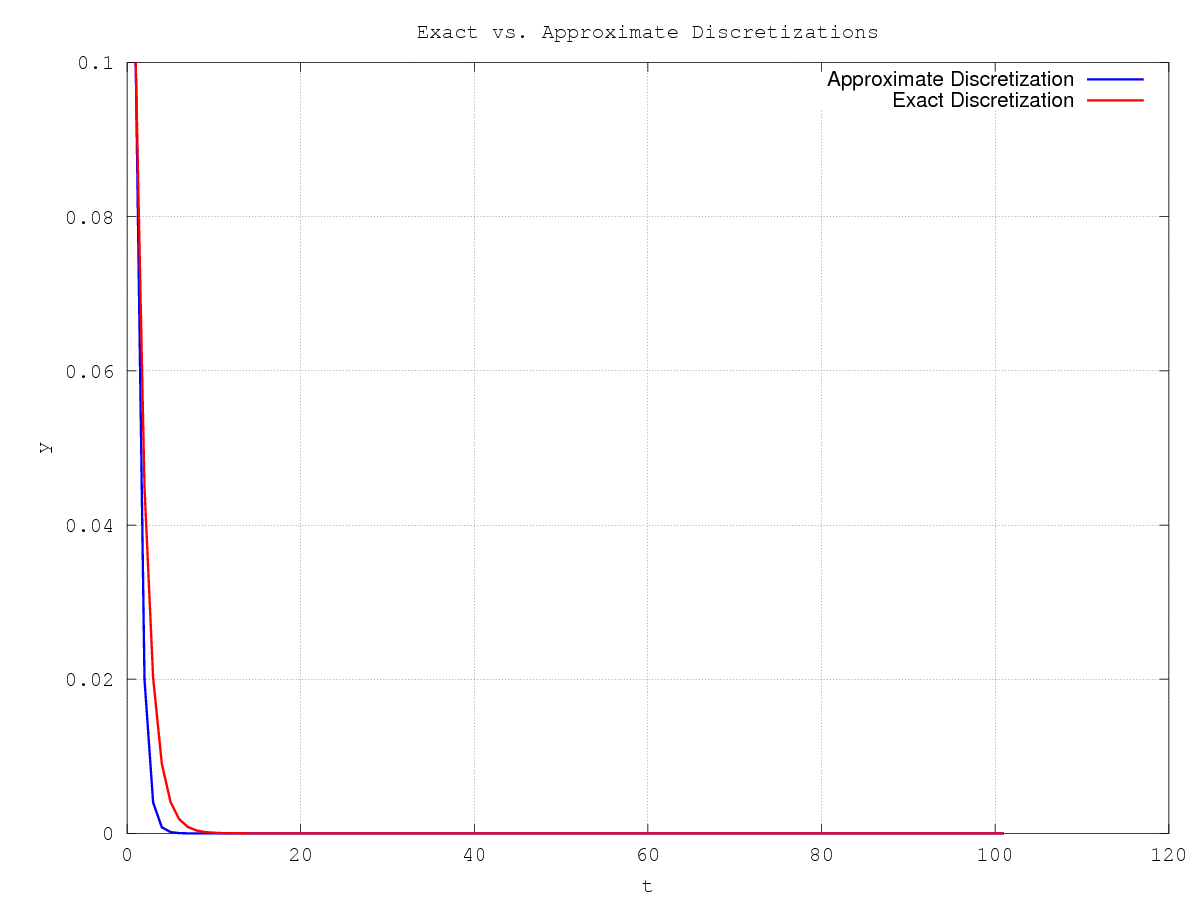
\includegraphics[scale=0.5]{figures/Question5Delta08.png} 
	          \label{fig:Q5Delta5}
	\caption{ $\delta = 0.8$  seconds}
	\end{figure}

	\begin{figure}[H]
			  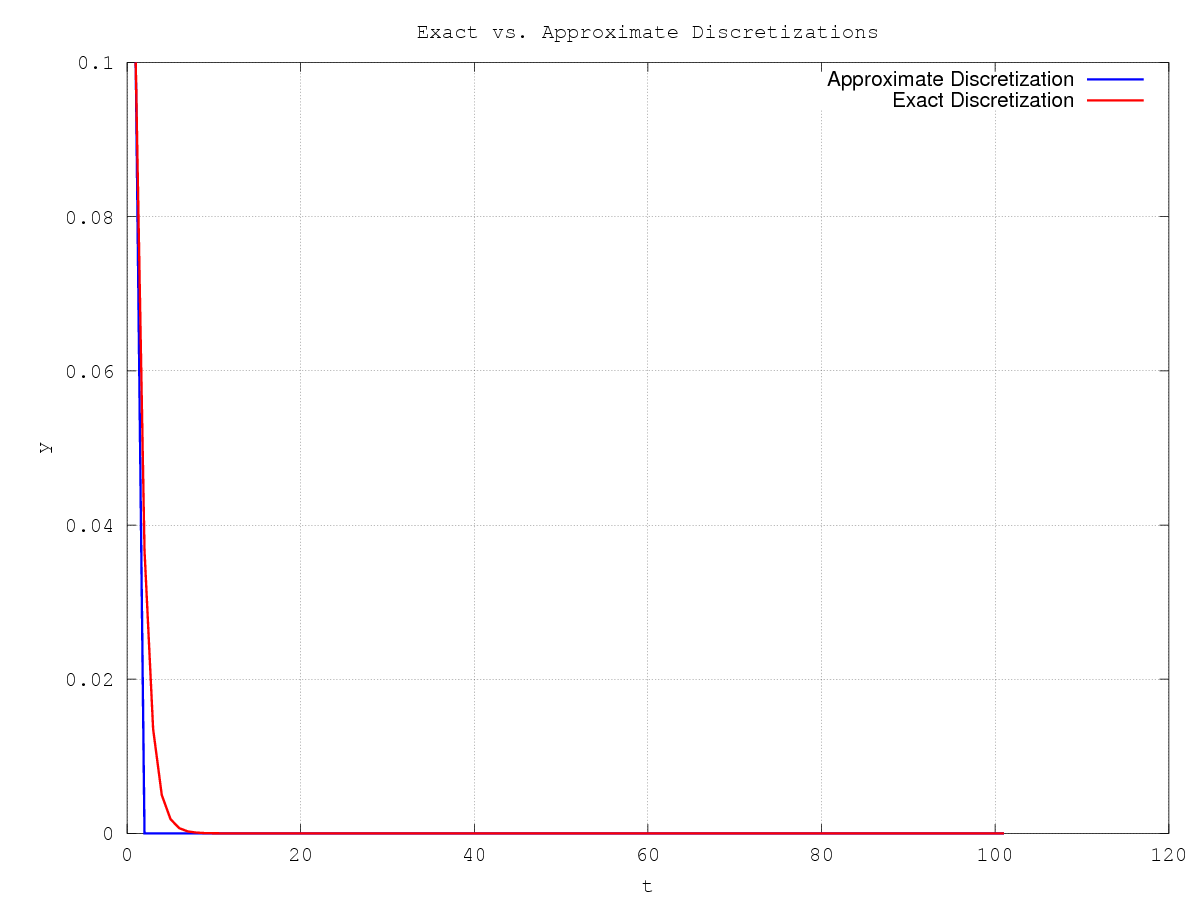
\includegraphics[scale=0.5]{figures/Question5Delta1.png} 
	          \label{fig:Q5Delta6}
	\caption{ $\delta = 1.0$  seconds}
	\end{figure}	
\end{center}	
\end{document}